
  
 
 \section{Caustics}
 \label{sec:appC-causticas}
 
  In this section will be present some properties of the billiard caustics.  Recall that is classically well known that the caustics of elliptic billiards are confocal ellipses (elliptic orbits) and confocal hyperbolas (billiard orbits pass between the two foci). See \cite[Chapter XI]{berger-2005}, \cite[Chapter 6]{hassel-2003}. 
  \begin{figure} 
	\begin{center}
	 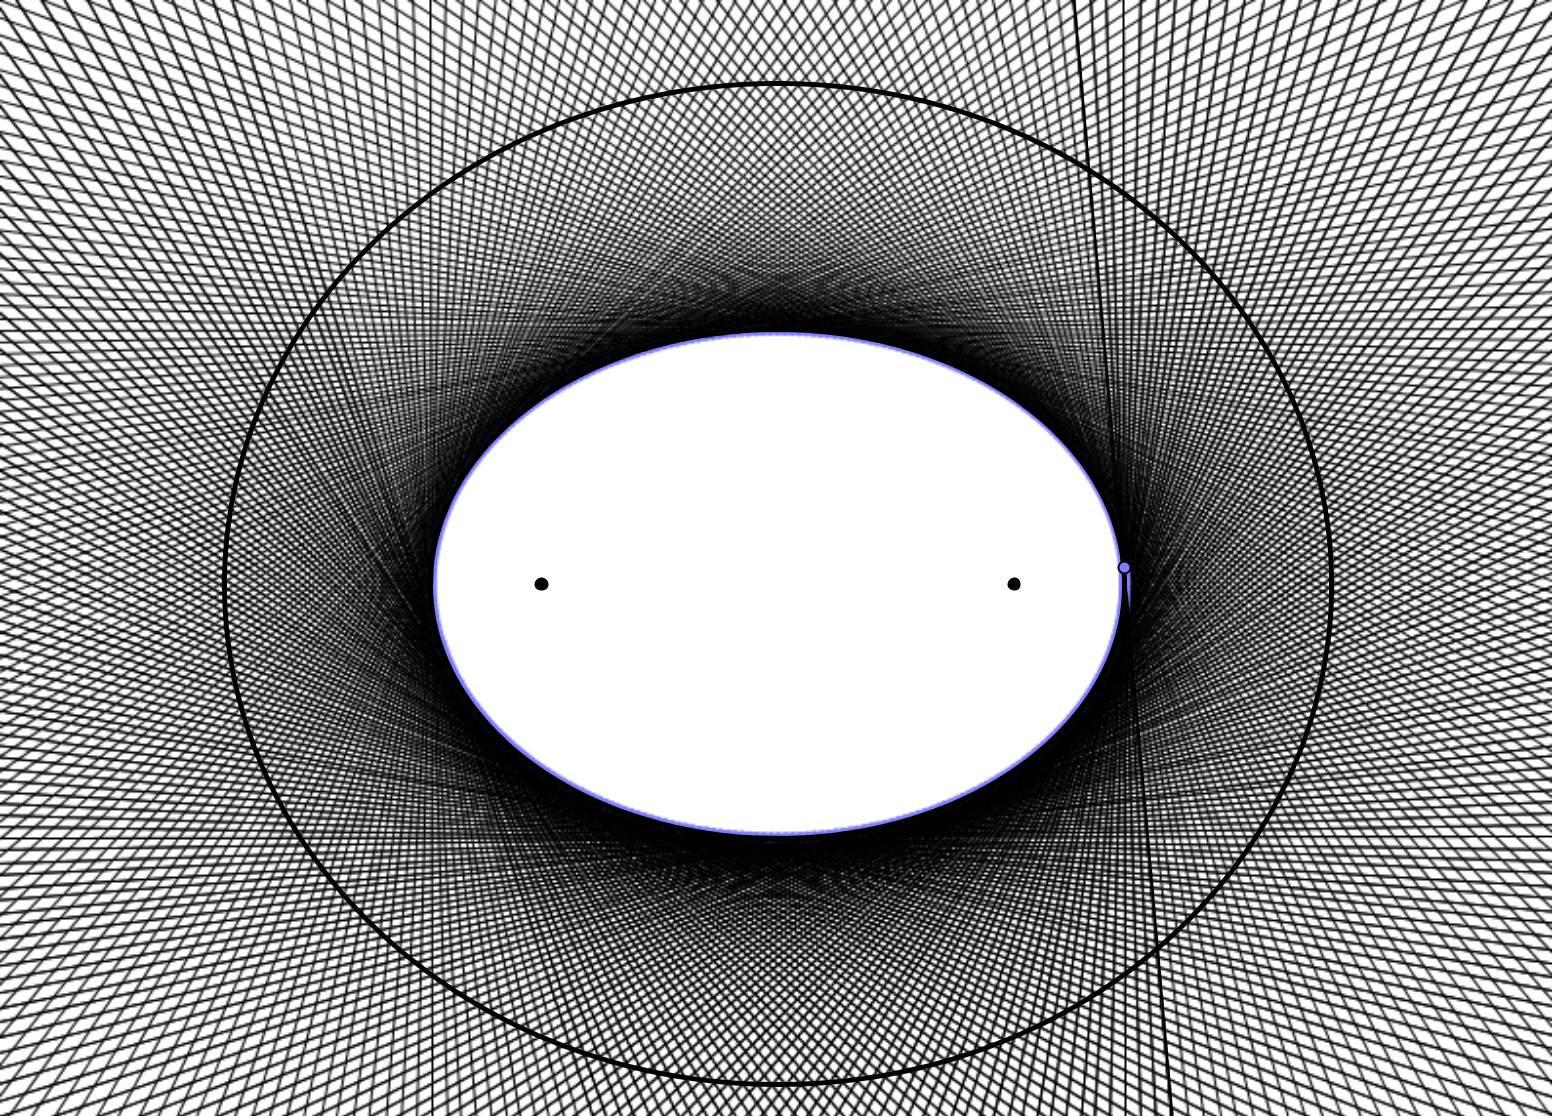
\includegraphics[scale=0.3]{zappC/pics/pics_appC_120_caustica_EH.png}
	 	 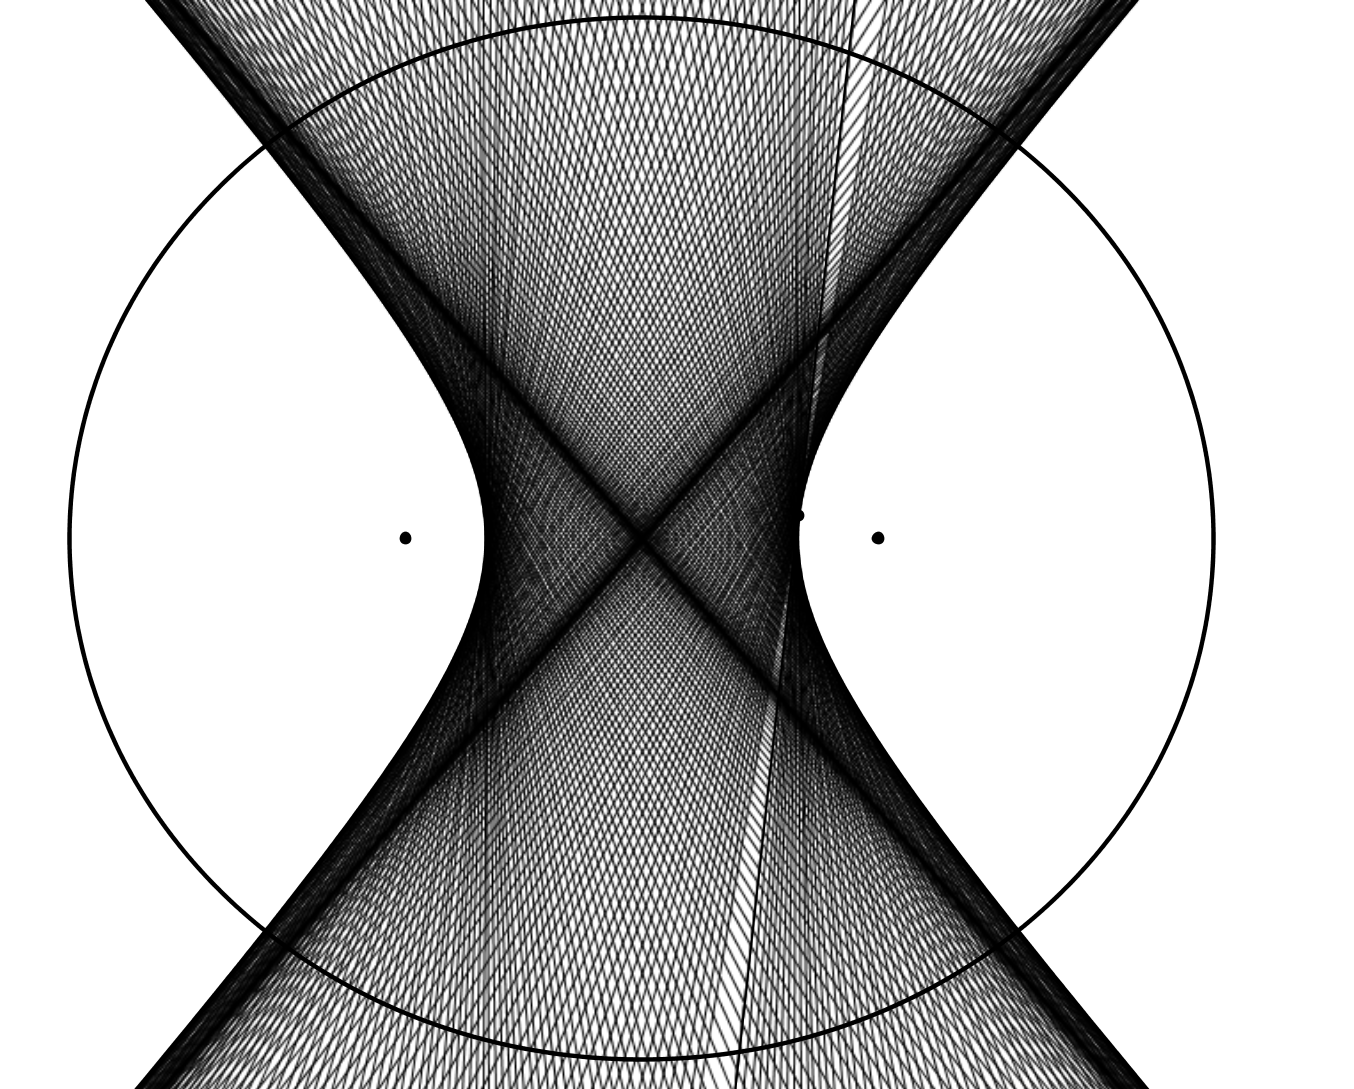
\includegraphics[scale=0.3]{zappC/pics/pics_appC_130_caustica_HE.png}
		\caption {Envelope of billiard orbits: ellipse (left) and hyperbola(right). \label{fig:envelope}}
	\end{center}
\end{figure}
 % Consider a smooth curve $\gamma$ and a lace streched
  
 % \begin{figure}[H]
%	\begin{center}
%		\def\svgwidth{0.55\textwidth}
	%	\input{otica.pdf_tex}
		%\includegraphics[angle=0, width=12cm]{bi.pdf}
%		\caption { . \label{fig:joachim}}
%	\end{center}
%\end{figure}
Let $\Gamma$ be a smooth convex curve parametrized by arc length $s$, and consider  a smooth family of oriented lines passing through the points of $\Gamma$. A parametric representation is given by
\[ \ell(s,v)= \Gamma(s)+ v d(s), \; |d(s)|=1,  \; |\Gamma'(s)|=1\]
Denote by $\theta(s)$ the angle between $d(s)$ and $\Gamma'(s)$. Therefore we can write
$d(s)=\cos\theta(s) T(s)+\sin\theta(s) N(s)$
where $\{T(s),N(s)\}$ is the Frenet frame of $\Gamma.$

 \begin{lemma}\label{lem:appC-envelope}
 The envelope of the family $\ell(s,v)$ is given by
 \[ E(s)=\Gamma(s)-\frac{\langle \Gamma'(s),d'(s)\rangle}{\langle d'(s),d'(s)\rangle} d(s).\]
\end{lemma}

\begin{proof} The envelope of a family of straight lines
is the locus of singularities and is defined by  the condition that the tangent vector of $E(s)=\ell(s,v(s))$ is parallel to $d'(s)$. Let  $[.,.]$ denotes the determinant of two vectors (oriented area of the parallelogram).
So it follows that
\[[E',d']=[\Gamma'(s)+v(s)d'(s)+v'(s)d(s),d'(s)]=0\]
    Then,
    \[ v(s)=-\frac{\langle \Gamma'(s),d'(s)\rangle}{\langle d'(s),d'(s)\rangle}\]
\end{proof}

Next, in other to apply to   billiards, consider the reflected family of lines defined by
\[\ell_r(s,u)= \Gamma(s)+u d_r(s), \; |d_r(s)|=1.\]

The envelope of $\ell_r(s,u)$ is defined by the function
\[ u(s)=-\frac{\langle \Gamma'(s),d_r'(s)\rangle}{\langle d_r'(s),d_r'(s)\rangle}.\]

\begin{proposition}\label{prop:appC-otica}
In the conditions above 
\begin{equation}
    \frac{1}{|u(s)|}+ \frac{1}{|v(s)|}=\frac{2k(s)}{sin\theta(s)}
\end{equation}
\end{proposition}

\begin{proof} We have that $d(s)=\cos\theta(s) T(s)+\sin\theta(s) N(s)$ and $d_r(s)=-\cos\theta(s) T(s)+\sin\theta(s) N(s).$
 
 Therefore,
 \[ \frac{1}{v(s)}=-\frac{\theta'(s)+k(s)}{\sin\theta(s)},\;\;\;\frac{1}{u(s)}=\frac{\theta'(s)-k(s)}{\sin\theta(s)}\]
 This ends the proof.
\end{proof}
  \begin{figure}[H]
	\begin{center}
		\def\svgwidth{0.75\textwidth}
	%		\input{corda3.pdf_tex}
	 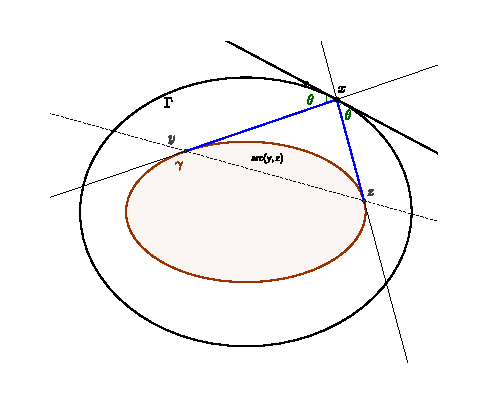
\includegraphics[scale=0.8]{zappC/pics/pics_appC_140_corda_comprimento.pdf}
		\caption {  Caustic and length of chords. \label{fig:appC-corda3}}
	\end{center}
\end{figure}

The following is a direct consequence of Proposition  \ref{prop:appC-otica}. See also \cite{katok3-1995}  and \cite{woj-1986}.

\begin{corollary}
    Consider a smooth convex curve $\Gamma$ with curvature $k>0.$ Let  $\gamma$ be the caustic and the chords as shown in Fig. \ref{fig:appC-corda3}. Then
    \[\frac{1}{|x-y|}+\frac{1}{|x-z|} =\frac{2k(x)}{\sin\theta}. \]
\end{corollary}

When the curve is not strictly convex we   have  the following consequence.  See \cite{mather-1984} and \cite[Chapter 3]{rozikov2018}.

\begin{theorem}   If the curvature of a convex smooth billiard curve vanishes at some point, then the associated billiard   map has no invariant circles.
 \end{theorem}

  \begin{theorem} Consider a convex billiard table with boundary $\Gamma$ of class $C^2$. Let $d$ be the diameter, $L$ be the length and $A$ be the area. Let 
   $k=\text{min}\{k(s)\}$ and $K=\text{max}\{k(s)\}$ of the curvature $k$ of $\Gamma$.  Suppose that $\lambda_1=\sqrt{2}d^2kK\leq 1$ and let $\lambda_2=1-\sqrt{2}kLd^2/A$. Then the billiard table contains a convex region, free of caustics, whose area is at least $\lambda_2$.\end{theorem}
   \begin{proof} See \cite{katok3-1995}.
   \end{proof}
   
     The result below can be found in   \cite[Lecture 10]{sinai-1977}. See also \cite{bialy-maxim-2018}, \cite[Lecture 28]{fuchs-2007} and \cite{gruber-1990}.
     
   \begin{proposition}\label{prop:caustic} Let $\gamma$ be a convex curve of length $l(\gamma)>0$.
   For $p$  outside $\gamma$ let $ L(p)$   the length of a string through $p$ stretched tightly around $\gamma$. For each $r>l(\gamma)$, let $C_r=\{p\in\mathbb{R}^2: L(p)=r\}.$ Then  $C_r$ is the  boundary of a convex body $\Gamma$ having $\gamma$ as a caustic.
      \end{proposition}
       \begin{figure}[H]
	\begin{center}
 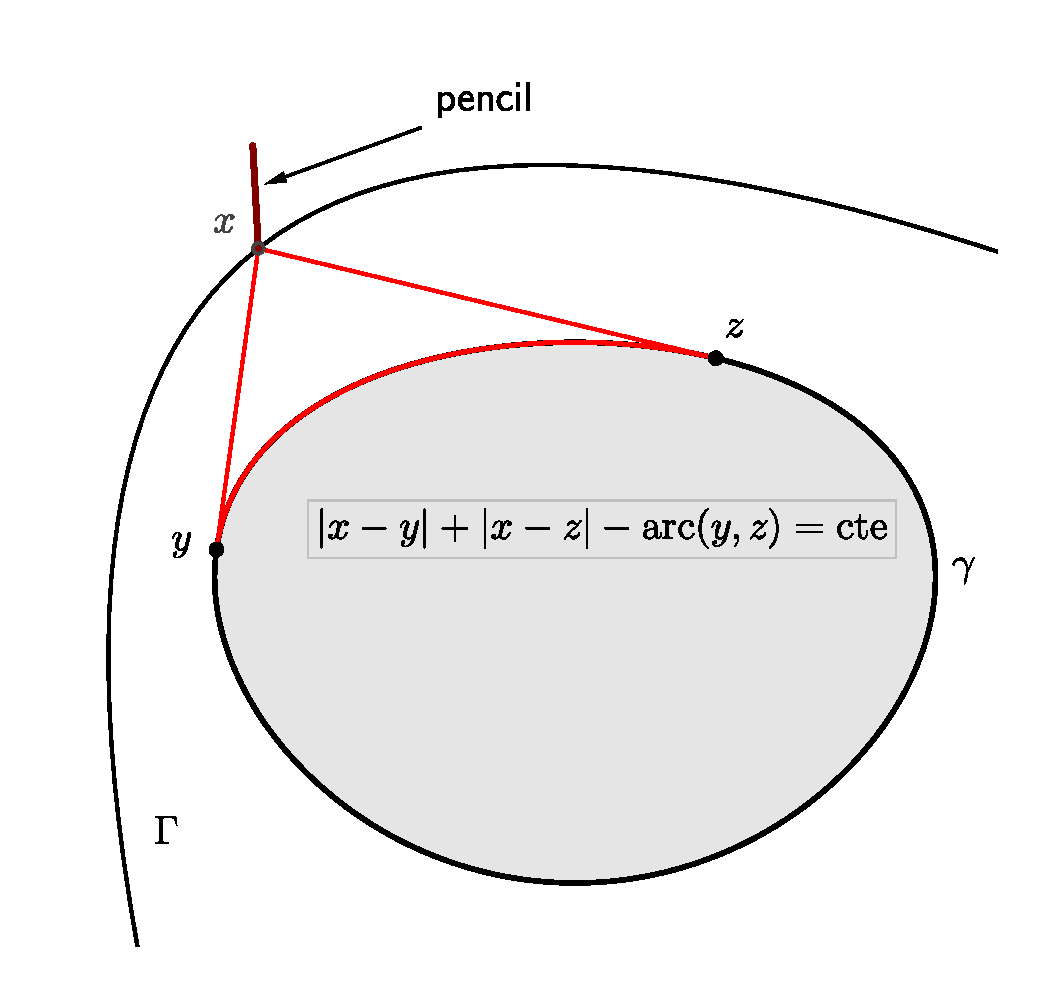
\includegraphics[scale=0.4]{zappC/pics/pics_appC_150_string_construcao.pdf}
		\caption {  Caustic $\gamma$ and the string construction of the outer  curve $\Gamma$. \label{fig:appC-caustica}}
	\end{center}
\end{figure}

  
   
   
    
   
   \begin{remark}
       The study of caustics of billiards on complex conics was developed in \cite{corentin2021-circum}. In this context it is used the   complex reflection law to define the billiard orbit.
   \end{remark}
      
 
 
